\documentclass[11pt]{article}
\usepackage{graphicx} % Required for inserting images
\usepackage{fontspec}
\usepackage[margin=3cm]{geometry}
\usepackage{xcolor}
\usepackage{fancyhdr}
\usepackage{ifthen}
\usepackage{sectsty}
\usepackage{hyperref}
\usepackage{colortbl}


% Colors
\definecolor{headBoxColor}{HTML}{eaf5fa}
\definecolor{headTextColor}{HTML}{8da5af}
\definecolor{lightgray}{HTML}{cecece}
\definecolor{midgray}{HTML}{808080}
\definecolor{nerfred}{HTML}{c00000}
\definecolor{darkblue}{HTML}{1a495d}
\definecolor{tablue}{HTML}{deeaf6}
\definecolor{red}{HTML}{ff0000}
\definecolor{gudgreen}{HTML}{90ee90}

% Format setup
\setmainfont{Lato}
\newfontfamily\titlfont{Roboto} % FIX THIS!!!!!!!!!!!!!!!!!!!!!!!!!!!!!!!!!!!
\newfontfamily\headfont{Lato}
\sectionfont{\fontsize{18}{22}\headfont\color{darkblue}}
\subsectionfont{\fontsize{16}{20}\headfont\color{darkblue}}
%\newcolumntype{C}[1]{>{\centering\arraybackslash}p{#1}}

% Title Page Vars
\def\Title{ANALYSIS}
\def\DocID{NAS-12345}
\def\Rev{IR}
\def\docDate{}
\def\Preparer{M. Doyle}
\def\Checker{}
\def\Approver{}

% Header/Footer
\pagestyle{fancy}
\fancyhf{}{}
\fancyfoot[R]{\textcolor{lightgray}{\rule{\linewidth}{0.1mm}}\\\textcolor{midgray}{\thepage\ |} \textcolor{lightgray}{Page}}
\renewcommand{\headrulewidth}{0pt}
\newlength{\stringWidth}
\settowidth{\stringWidth}{\textbf{\DocID}}
\fancyhead[L]{\fcolorbox{headBoxColor}{headBoxColor}{\textcolor{headTextColor}{ \textbf{\DocID}\rule{\dimexpr\linewidth - \stringWidth\relax}{0pt}}}}
\fancyhead[R]{\fcolorbox{headBoxColor}{headBoxColor}{\textcolor{headTextColor}{\textbf{\Title}}}}



\begin{document}

\begin{titlepage}
\centering
\vspace*{100pt}
\begin{figure}[h!]

\includegraphics[width=1\linewidth]{images/NAS.png}
\end{figure}

\vspace{130pt}

{\fontsize{30}{36} \titlfont \Title}

\vspace{70pt}

{\fontsize{30}{36} \titlfont \DocID\ REV. \Rev}

\vspace{10pt}

\ifx\docDate\empty
  \today
\else
  \docDate
\fi

\begin{table}[b]
    \centering
    \begin{tabular}{|l|l|}
        \hline Prepare\rule{30pt}{0pt} & \Preparer\rule{50pt}{0pt} \\
        \hline Check & \Checker\\
        \hline Approve & \Approver\\\hline
    \end{tabular}
\end{table}
\end{titlepage}
\setcounter{page}{1}

\section{Introduction}

Yadda yadda.
%ellStart
\clearpage
\section{Ellipse}

Ellipse analysis in Table \ref{tab:EA1}:

\begin{table}[h]
    \centering
    \begin{tabular}{|l|l|l|l|l|}
        \hline \rowcolor{tablue} \textbf{$\eta$ (Deg)} & \textbf{$\eta$ (Rad)} & \textbf{$F_\epsilon$} & \textbf{$F_\eta$} & \textbf{$F_{\epsilon\eta}$}\\\hline
		{\%ellTLH}
    \end{tabular}
	\caption{Ellipse Analysis}
	\label{tab:EA1}
\end{table}

Graph seen in Figure \ref{fig:EA1}:

\begin{figure}[]
\label{fig:EA1}
\includegraphics[width=1\linewidth]{temp/ellipse_chart_b64png.png}
\caption{Ellipse Graph}
\end{figure}
%ellEnd
%TCStart
\clearpage
\section{Tension Clip}

Tension clip analysis within.

\subsection{Data}

Data seen below.

\begin{table}[!ht]
    \centering
	\label{tab:D4_1}
	\caption{Data From BM7024.01.03.03 Figure 4.1}
    \begin{tabular}{|l|l|l|l|l|l|l|l|l|l|}
    \hline
        c            t & 0.020  & 0.032  & 0.040  & 0.050  & 0.063  & 0.071  & 0.080  & 0.090  & 0.1 \\ \hline
        0.4 & 25.68  & 69.41  & 108.47  & 166.28  & 262.38  & 337.38  & 425.65  & 536.16  & 665.99  \\ \hline
        0.5 & 21.74  & 55.31  & 86.56  & 135.00  & 210.00  & 270.93  & 342.03  & 432.04  & 533.71  \\ \hline
        0.75 & 13.84  & 34.92  & 56.01  & 88.04  & 139.61  & 177.89  & 226.33  & 286.33  & 354.37  \\ \hline
        1 & 9.85  & 27.03  & 41.88  & 66.88  & 106.72  & 134.06  & 172.34  & 214.92  & 266.54  \\ \hline
        1.25 & 7.43  & 22.27  & 34.77  & 51.95  & 85.55  & 107.42  & 136.33  & 174.02  & 213.12  \\ \hline
        1.5 & 6.57  & 17.50  & 28.44  & 43.28  & 68.28  & 87.81  & 112.03  & 140.93  & 175.35  \\ \hline
        1.75 & 4.93  & 14.30  & 25.24  & 37.74  & 58.05  & 76.02  & 97.11  & 121.93  & 152.43  \\ \hline
        2 & 5.63  & 12.66  & 21.25  & 30.63  & 50.16  & 65.78  & 84.53  & 106.84  & 133.43 \\ \hline
    \end{tabular}
\end{table}

\begin{figure}[h!]
    \centering
    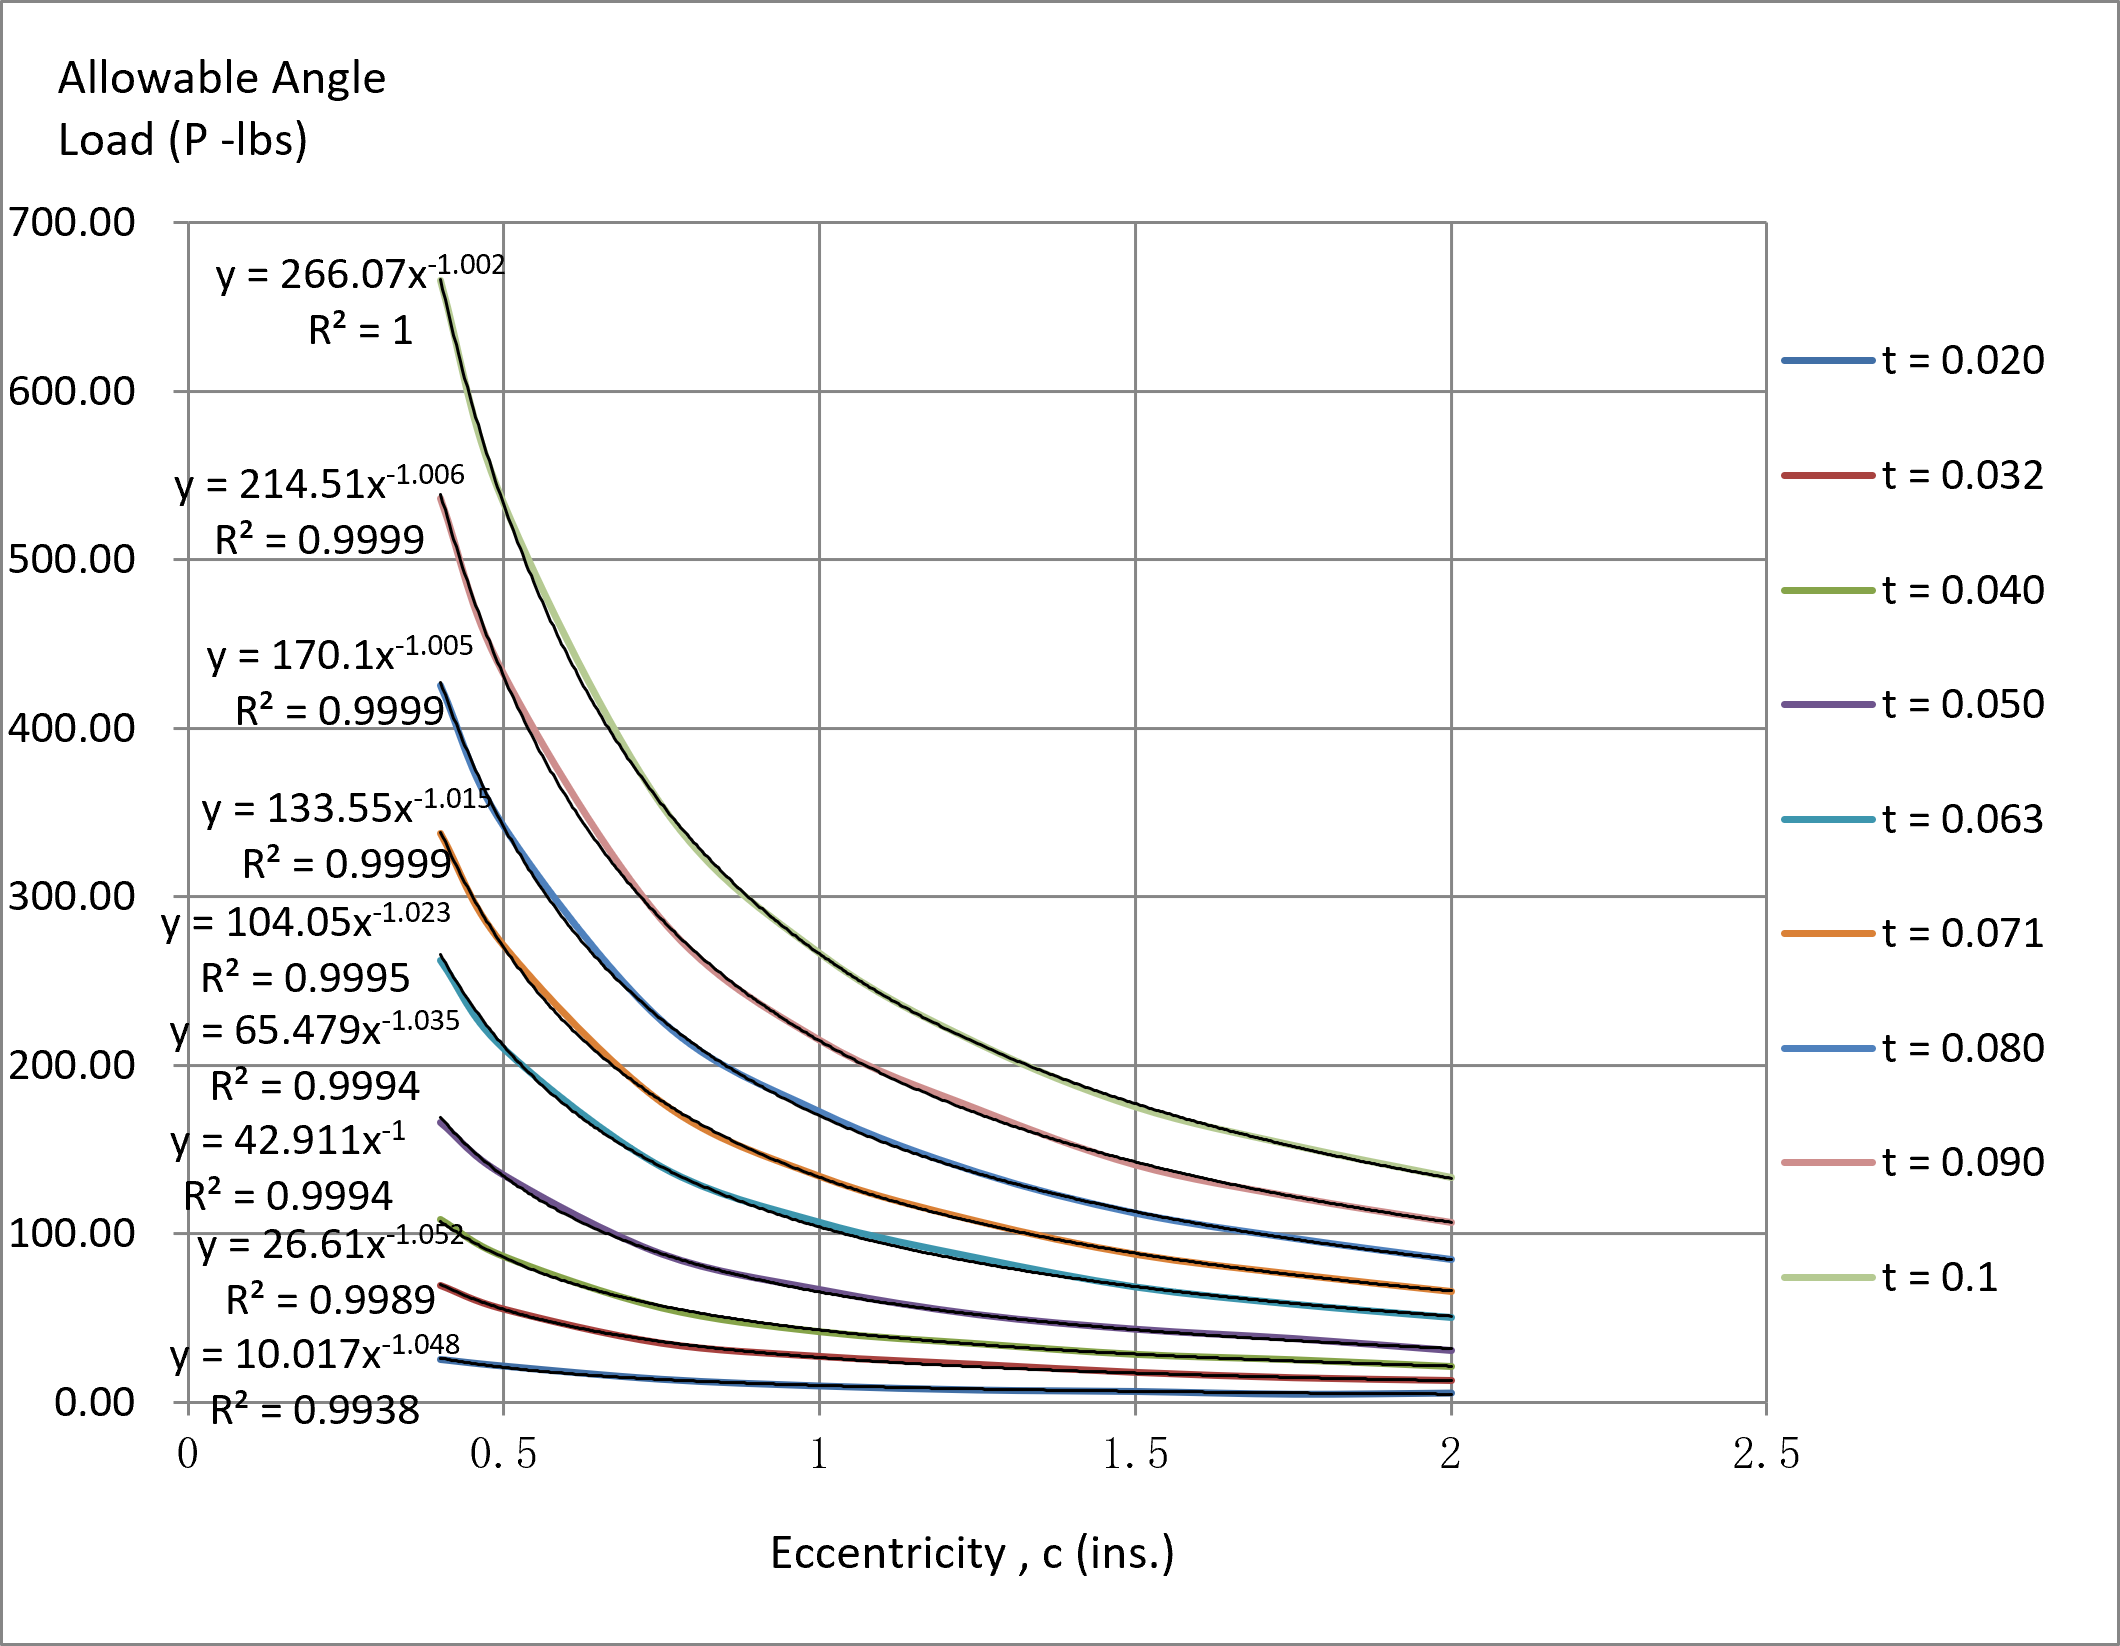
\includegraphics[width=0.9\linewidth]{images/tension_clip/UAL_CSMA.png}
    \label{fig:UAL1}
\end{figure}

\begin{table}[!ht]
    \centering
	\label{tab:D4_2}
	\caption{Data From BM7024.01.03.03 Figure 4.2}
    \begin{tabular}{|l|l|l|l|l|l|l|}
    \hline
        c            t & 0.060  & 0.090  & 0.125  & 0.160  & 0.200  & 0.250  \\ \hline
        0.4 & 215 & 495 & 950 & 1580 & 2495 & 3995 \\ \hline
        0.5 & 175 & 400 & 772.5 & 1275 & 1995 & 3130 \\ \hline
        0.75 & 115 & 260 & 505 & 845 & 1325 & 2090 \\ \hline
        1 & 95 & 200 & 380 & 625 & 995 & 1550 \\ \hline
        1.25 & 67.5 & 152.5 & 305 & 500 & 790 & 1240 \\ \hline
        1.5 & 53.5 & 135 & 252.5 & 412.5 & 650 & 1030 \\ \hline
        1.75 & 51.5 & 112.5 & 215 & 350 & 555 & 875 \\ \hline
        2 & 50 & 102.5 & 195 & 312.5 & 495 & 770 \\ \hline
    \end{tabular}
\end{table}

\begin{figure}[h!]
    \centering
    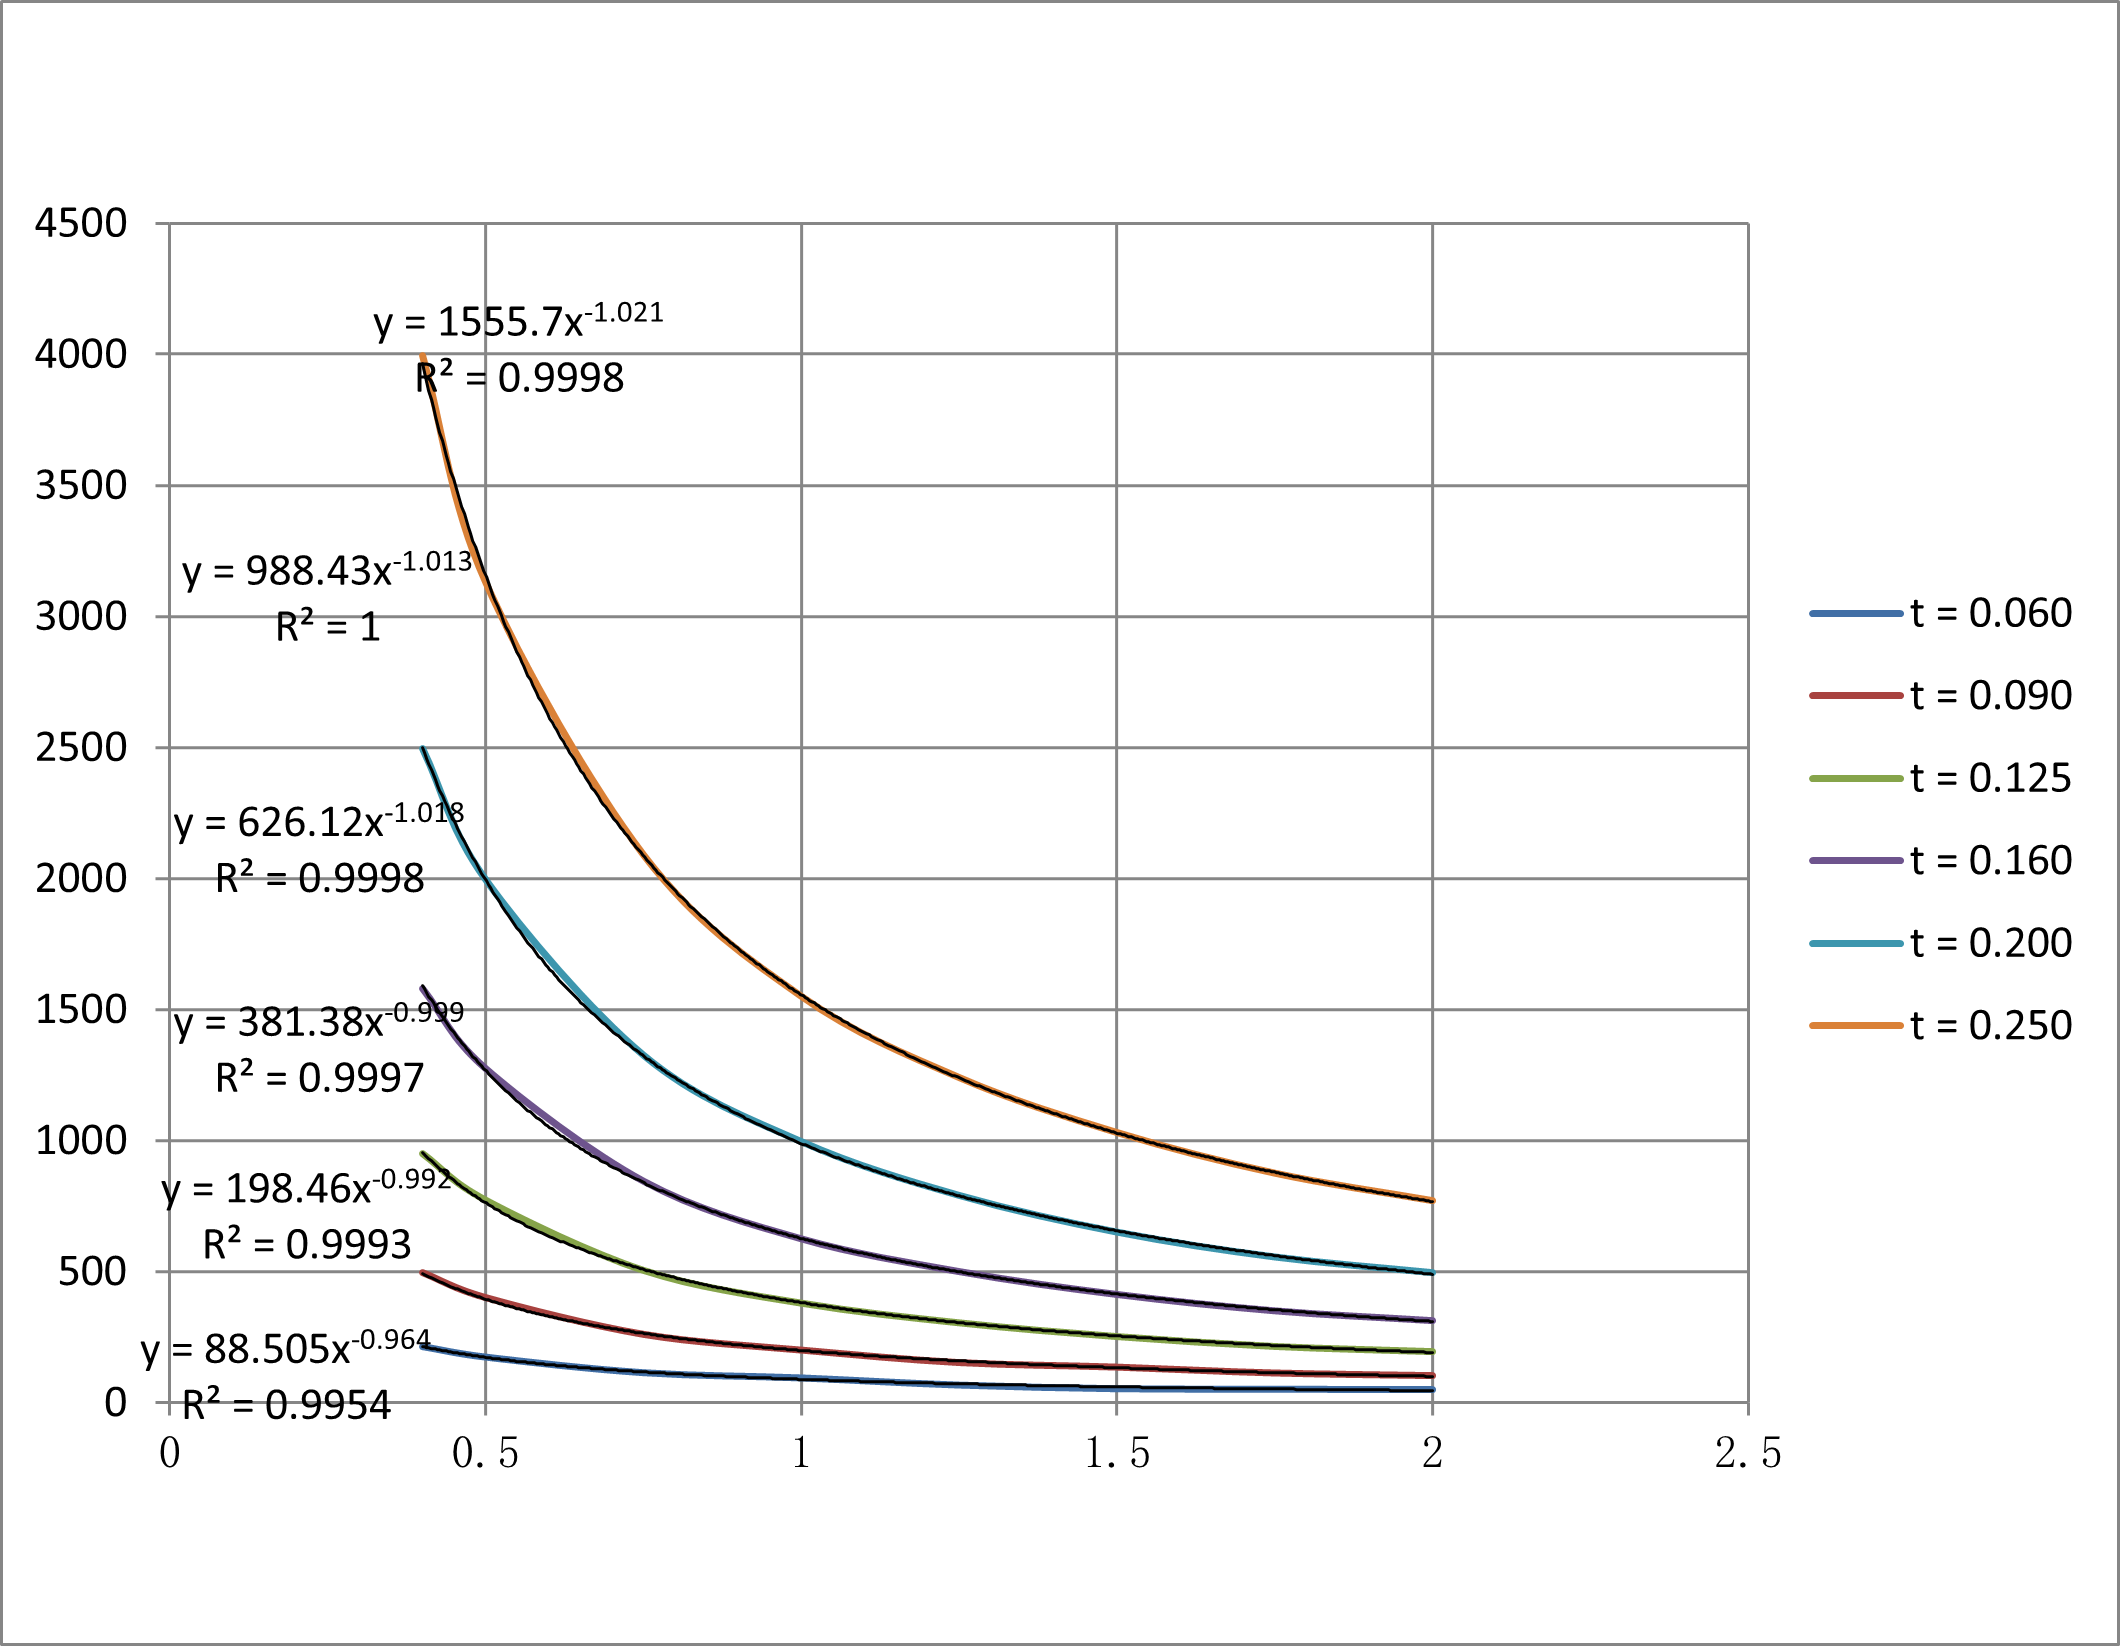
\includegraphics[width=0.9\linewidth]{images/tension_clip/UAL_EA.png}
    \label{fig:UAL2}
\end{figure}

\clearpage

\subsection{Analysis}

Input parameters in Table \ref{tab:TC1}.

\begin{table}[h]
    \centering
    \begin{tabular}{|l|l|l|l|l|l|l|}
        \hline \textbf{Clip Type} & \textbf{$t$} & \textbf{$c$} & \textbf{$F_{cy}$} & \parbox[c]{3cm}{\textbf{Attachment Point Spacing}} & \textbf{Angle Width} & \parbox[c]{3cm}{\textbf{Attachment Point Count}}\\\hline
        {\%CTIn} & {\%tIn} & {\%cIn} & {\%FcyIn} & {\%PSIn} & {\%AWIn} & {\%PCIn}\\\hline
    \end{tabular}
	\caption{Input parameters}
	\label{tab:TC1}
\end{table}

The above parameters result in an ultimate allowable load of \textbf{{\%POut}}.
%TCEnd
%cripStart
\clearpage
\section{Crippling}

Crippling analysis within.

$F_{CY}={\%Fcy}$, $E_C={\%Ec}$, data in Table \ref{tab:crip1}:

\begin{table}[h]
    \centering
    \begin{tabular}{ccccccc}
        \textcolor{darkblue}{\textbf{Flange}} & \textcolor{darkblue}{\textbf{b}} & \textcolor{darkblue}{\textbf{t}} & \textcolor{darkblue}{\textbf{Edges}} & \textcolor{darkblue}{\textbf{Area}} & \textcolor{darkblue}{\textbf{Fcc}} & \textcolor{darkblue}{\textbf{Fcc*A}}\\\hline
        1 & {\%b1} & {\%t1} & {\%Edges1} & {\%A1} & {\%Fcc1} & {\%FccA1}\\
        2 & {\%b2} & {\%t2} & {\%Edges2} & {\%A2} & {\%Fcc2} & {\%FccA2}\\
    \end{tabular}
	\caption{Crippling data}
	\label{tab:crip1}
\end{table}

The ultimate combined allowables evaluate to: \[F_{CC}={\%Fcc}, P_{CC}={\%Pcc}\]
%cripEnd
%bCripStart
\clearpage
\section{Bending Crippling}

Bending crippling analysis within.

$F_{CY}={\%Fcy}$, $E_C={\%Ec}$, data in Table \ref{tab:bCrip1}:

\begin{table}[h]
    \centering
    \begin{tabular}{ccccccccc}
        \textcolor{darkblue}{\textbf{Flange}} & \textcolor{darkblue}{\textbf{Type}} & \textcolor{darkblue}{\textbf{b}} & \textcolor{darkblue}{\textbf{t}} & \textcolor{darkblue}{\textbf{Edges}} & \textcolor{darkblue}{\textbf{$\overline{Y}$}} & \textcolor{darkblue}{\textbf{$F_{CC}$}} & \textcolor{darkblue}{\textbf{$Y_i$}} & \textcolor{darkblue}{\textbf{$M_o$}}\\\hline
        1 & {\%Type1} & {\%b1} & {\%t1} & {\%Edges1} & {\%Ybar1} & {\%Fcc1} & {\%Yi1} & {\%Mo1}\\
        2 & {\%Type2} & {\%b2} & {\%t2} & {\%Edges2} & {\%Ybar2} & {\%Fcc2} & {\%Yi2} & {\%Mo2}\\
    \end{tabular}
	\caption{Bending crippling data}
	\label{tab:bCrip1}
\end{table}

The maximum allowable moment evaluates to: \[Max Allowable Moment={\%MAM}\]
%bCripEnd
%OFBStart
\clearpage
\section{Outstanding Flange Buckling}

Outstanding flange buckling analysis within. Input data in Table \ref{tab:OFB1}, output data in Table \ref{tab:OFB2}. {\%ASS}

\begin{table}[h]
    \centering
    \makebox[\textwidth]{
    \scalebox{0.9}{ % Scale down to 70%
    \begin{tabular}{|c|cccccccccccc|}
      \hline \textbf{Section} & \textbf{Material} & \textbf{$E_C$ (msi)} & \textbf{$F_{CY}$ (ksi)} & \textbf{$\mu$} & \textbf{$nc$} & \textbf{$t$ (in)} & \textbf{$b$ (in)} & \textbf{$F_0$ (psi)} & \textbf{$F_f$ (psi)} & \textbf{$t_{web}$ (in)} & \textbf{$H_{fr}$ (in)} & \textbf{Lst/Pitch Ratio}\\\hline
        1 & {\%Mater} & {\%Ec} & {\%Fcy} & {\%mu} & {\%nc} & {\%t} & {\%b} & {\%F0} & {\%Ff} & {\%tweb} & {\%Hfr} & {\%LPR}\\\hline
    \end{tabular}}}
	\caption{Input data}
	\label{tab:OFB1}
\end{table}


\begin{table}[h]
    \centering
    \begin{tabular}{|c|cccccc|cc|}
      \hline \textbf{Section} & \textbf{$F_0/F_f$} & \textbf{$K$} & \textbf{$E_t$ (psi)} & \textbf{$E_s$ (psi)} & \textbf{$\eta$} & \textbf{$\mu_c$ (lb/in$\cdot$rad)} & \textbf{$F_{ofb}$ (psi)} & \textbf{$MS$}\\\hline
      1 & {\%F0/Ff} & {\%K} & {\%Et} & {\%Es} & {\%eta} & {\%mu\_c} & {\%Fofb} & {\%MS}\\\hline
    \end{tabular}
	\caption{Output data}
	\label{tab:OFB2}
\end{table}

%OFBEnd
%FPBStart
\clearpage
\section{Flat Plate Buckling}

Flat plate buckling analysis within. Input data in Table \ref{tab:FPB1}, output data in Table \ref{tab:FPB2}.

\begin{table}[h]
    \centering
    \begin{tabular}{|c|c|c|c|c|c|c|c|c|}
      \hline \textbf{Edge Type} & $f_S$ & $a$ & $b$ & $t$ & $E_C$ & $\nu$ & $f_1$ & $f_2$\\\hline
      {\%ET} & {\%fs} & {\%a} & {\%b} & {\%t} & {\%Ec} & {\%nu} & {\%f1} & {\%f2}\\\hline
    \end{tabular}
	\caption{Input data}
	\label{tab:FPB1}
\end{table}

\begin{table}[h]
    \centering
     \makebox[\textwidth]{
    \scalebox{0.9}{
    \begin{tabular}{|c|c|c|c|c|c|c|c|c|c|c|c|}
      \hline \multicolumn{4}{|c|}{Shear Buckling Alone} & \multicolumn{4}{c|}{Compression/Bending Buckling Alone} & \multicolumn{4}{c|}{Margin due to Combined Loading}\\\hline 
	  $a/b$ & $K_S$ & $F_{SCR}$ (ksi) & \textbf{MS} & $f_2/f_1$ & $K_C$ & $F_{CR}$ (ksi) & \textbf{MS} & $f_S/F_{SCR}$ & $f_1/F_{CR}$ & $f_2/f_1$ & \textbf{MS}\\\hline
      {\%ab} & {\%Ks} & {\%Fscr} & \cellcolor{<MS1>}{\%MS\_SBA} & {\%f2f1} & {\%Kc} & {\%Fcr} & \cellcolor{<MS2>}{\%MS\_CBA} & {\%fsFscr} & {\%f1Fcr} & {\%f2f1} & \cellcolor{<MS3>}{\%MS\_MCL}\\\hline
    \end{tabular}}}
	\caption{Output data}
	\label{tab:FPB2}
\end{table}

\begin{figure}[h]
\label{fig:FPB1}
\includegraphics[width=1\linewidth]{temp/FPB_chart1_b64png.png}
\caption{Buckling Stress Coefficients for Flat Plates Loaded in Uniform Shear}
\end{figure}

\begin{figure}[h]
\label{fig:FPB2}
\includegraphics[width=1\linewidth]{temp/FPB_chart2_b64png.png}
\caption{Buckling Stress Coefficients for Flat Plates Under Bending, Compression or Tension}
\end{figure}

\begin{figure}[h]
\label{fig:FPB3}
\includegraphics[width=1\linewidth]{temp/FPB_chart3_b64png.png}
\caption{Initial Buckling of Flat Plates Under Compression, Bending and Shear}
\end{figure}

%FPBEnd
\clearpage
\section{Conclusion}

Mhm.

\end{document}